\part{kai}
 \begin{frame}
 	\frametitle{Inhalt}
 	\tableofcontents[%
% 		currentsection, % causes all sections but the current to be shown in a semi-transparent way.
% % 		currentsubsection, % causes all subsections but the current subsection in the current section to ...
% % 		hideallsubsections, % causes all subsections to be hidden.
% 		hideothersubsections, % causes the subsections of sections other than the current one to be hidden.
% % 		part=, % part number causes the table of contents of part part number to be shown
 	%	pausesections, % causes a \pause command to be issued before each section. This is useful if you
% 		pausesubsections, %  causes a \pause command to be issued before each subsection.
% % 		sections={ overlay specification },
 ]
 \end{frame}
%hier gehts los

\section{TikZ}
\begin{frame}
\frametitle{Umgebung}
\begin{itemize}
  \item Zum Zeichnen unter \LaTeX wird nachfolgend TikZ verwendet
  \item die Zeichenumgebung wird mit $\backslash$ begin\{tikzpicture\} begonnen
\end{itemize}
\end{frame}

\begin{frame}
\frametitle{Kreise}
\begin{table}[!h]
\begin{tabular}{lr}

$\backslash$begin\{tikzpicture\} & \\
\\
$\backslash$path[draw] (0,0) circle (2ex) 
&

\begin{tikzpicture}
  \path[draw] (0,0) circle (2ex);
\end{tikzpicture} 
\\  
\\
$\backslash$path[fill] (0,-2) circle (2ex) 
&

\begin{tikzpicture}
  \path[fill] (0,0) circle (2ex);
\end{tikzpicture}
\\
\\
$\backslash$path[fill=yellow, draw=red] (0,-4) circle (2ex)
&

\begin{tikzpicture}
  \path[fill=yellow,draw=red] (0,0) circle (2ex);
\end{tikzpicture}
\\
\\
$\backslash$end\{tikzpicture\} & \\
\end{tabular}
\end{table}
\end{frame}

\begin{frame}
\frametitle{Diagramme}
\begin{figure}[!h]
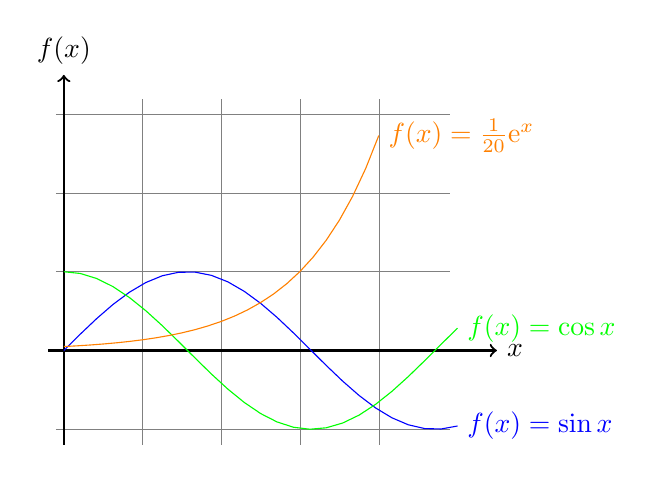
\begin{tikzpicture}[domain=0:5]
  \draw[very thin,color=gray] (-0.1,-1.2) grid (4.9,3.2);
  \draw[->,thick] (-0.2,0) -- (5.5,0) node[right] {$x$};
  \draw[->,thick] (0,-1.2) -- (0,3.5) node[above] {$f(x)$};
  \draw[color=blue] plot (\x,{sin(\x r)}) node[right] {$f(x) = \sin x$};
  \draw[color=green] plot (\x,{cos(\x r)}) node[right] {$f(x) = \cos x$};
  \draw[color=orange,domain=0:4] plot (\x,{0.05*exp(\x)}) node[right] {$f(x) = \frac{1}{20} \mathrm e^x$};
\end{tikzpicture}


\end{figure}
\end{frame}

\begin{frame}
\frametitle{Diagramme}
	\lstsettex
	\lstinputlisting{./listings/diagram.tex}
\end{frame}

\begin{frame}
\frametitle{Graphen}
\begin{figure}[!h]
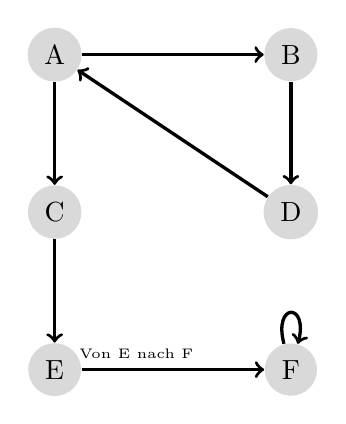
\begin{tikzpicture}
  \node (A) at (0, 4) [circle, fill=gray!30] {A};
  \node (B) at (3, 4) [circle, fill=gray!30] {B};
  \node (C) at (0, 2) [circle, fill=gray!30] {C};
  \node (D) at (3, 2) [circle, fill=gray!30] {D};
  \node (E) at (0, 0) [circle, fill=gray!30] {E};
  \node (F) at (3, 0) [circle, fill=gray!30] {F};

  \draw[->, very thick] (A) to (B);
  \draw[->, very thick] (B) to (D);
  \draw[->, very thick] (D) to (A);
  \draw[->, very thick] (A) to (C);
  \draw[->, very thick] (C) to (E);
  \draw[->, very thick] (E) to node[pos=0.3,above] {\tiny{Von E nach F}} (F);
  \draw[->, very thick] (F) to[loop above] (F);
\end{tikzpicture}

\end{figure}
\end{frame}

\begin{frame}
\frametitle{Graphen}
	\lstsettex
	\lstinputlisting{./listings/graph.tex}
\end{frame}

\begin{frame}
\frametitle{Feistel}
\begin{figure}[!h]
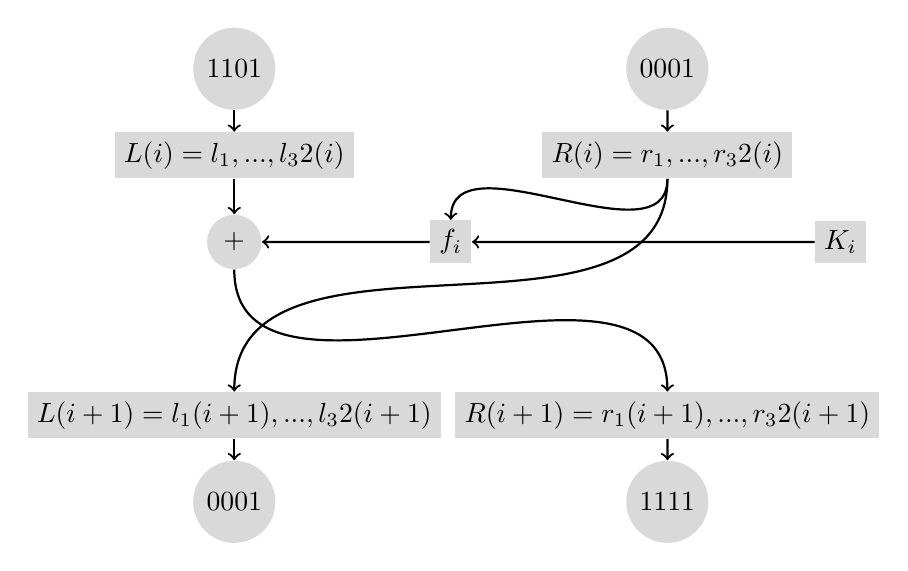
\begin{tikzpicture}[scale=1.1]
  \node [circle, fill=gray!30] (c1) at (0, 0) {$ 0001 $};
  \node [circle, fill=gray!30] (c2) at (5, 0) {$ 1111 $};
  \node (a1) at (0,1) [fill=gray!30] {$L(i+1)=l_1 (i+1), ... ,l_32(i+1)$};
  \node (a2) at (5,1) [fill=gray!30] {$R(i+1)=r_1 (i+1), ... ,r_32(i+1)$};
  \node (a3) at (0,4) [fill=gray!30] {$L(i)=l_1 , ... , l_32 (i)$};
  \node (a4) at (5,4) [fill=gray!30] {$R(i)=r_1 , ... , r_32 (i)$};
  \node [circle, fill=gray!30] (c3) at (0, 5) {$ 1101 $};
  \node [circle, fill=gray!30] (c4) at (5, 5) {$ 0001 $};
  \node [circle, fill=gray!30] (c5) at (0, 3) {$ + $};
  \node (a5) at (2.5,3) [fill=gray!30] {$f_i$};
  \node (a6) at (7,3) [fill=gray!30] {$K_i$};

  \draw[->, thick] (c3) to (a3);
  \draw[->, thick] (c4) to (a4);
  \draw[->, thick] (a3) to (c5);
  \draw[->, thick] (a1) to (c1);
  \draw[->, thick] (a2) to (c2);
  \draw[->, thick] (a6) to (a5);
  \draw[->, thick] (a5) to (c5);
  \draw[->, thick] (c5) to[out=-90, in=90] (a2)  ;
  \draw[->, thick] (a4) to[out=-90, in=90] (a1)  ;
  \draw[->, thick] (a4) to[out=-90, in=90] (a5)  ;
\end{tikzpicture}

\end{figure}
\end{frame}

\begin{frame}
\frametitle{Feistel}
	\lstsettex
	\lstinputlisting{./listings/feistel.tex}
\end{frame}

